%&pdfLaTeX
% !TEX encoding = UTF-8 Unicode
\documentclass{article}
\usepackage{ifxetex}
\ifxetex
\usepackage{fontspec}
\setmainfont[Mapping=tex-text]{STIXGeneral}
\else
\usepackage[T1]{fontenc}
\usepackage[utf8]{inputenc}
\fi
\usepackage{textcomp}

\usepackage{graphicx}
\usepackage{array}
\usepackage{amssymb}
\usepackage{fancyhdr}
\renewcommand{\headrulewidth}{0pt}
\renewcommand{\footrulewidth}{0pt}
\usepackage{color}

\pagestyle{fancy}
\rhead{}
\rfoot{}
\chead{}
\cfoot{}
\fancyhead[LO]{
 { Commercial in Confidence}}
\fancyfoot[LE]{\thepage{}}
\fancyfoot[LO]{\thepage{}}
\definecolor{color01}{rgb}{0.00,0.00,0.00}
\definecolor{color06}{rgb}{1.00,0.00,0.00}
\definecolor{color19}{rgb}{0.00,0.19,0.33}
\definecolor{color25}{rgb}{0.12,0.29,0.49}
\newcommand{\nep}{\textsc{NEPTUNE}}
\newcommand{\exc}{\textsc{E}x\textsc{CALIBUR}}
\newcommand{\Papp}{Proxyapp}
\newcommand{\papp}{proxyapp}


\begin{document}

%%\begin{figure}[htbp]

\includegraphics[width=950pt, height=570pt, keepaspectratio=true]{../corpics/binwall.png}
%%\caption{This should be the caption for \texttt{M3.3.1-fig001.jpg}.}
%%\end{figure}

%%\begin{figure}[htbp]

\includegraphics[width=31pt, height=29pt, keepaspectratio=true]{../corpics/UKAEA-arms.png}
%%\caption{This should be the caption for \texttt{M3.3.1-fig002.png}.}
%%\end{figure}

{\huge{}{ \textbf{\exc \   }}}

{\huge{}{ \textbf{\nep \  : Background Information and User Requirements 
for Design patterns}}}

{\huge{}{ \textbf{M3.3.1}}}

\baselineskip=12pt
\textbf{Abstract}

This report describes the work carried out for the \nep \   project at Milestone 3.3.1 
towards deliverable D3.1 ``Module Guide document''. This is a review of the design 
challenges and of the available solutions for the tokamak edge codes 
starting from coupled workflows and going on to parallel hardware. 
\pagebreak


\section{Introduction}

The physics of the tokamak edge requires a multiscale approach due to the coupling 
of the space and time scales over a wide dynamic range (from fractions of millisecond 
to seconds and from mm to meters). At the same 
time, a multi-physics approach is required for the edge region where plasma, neutral 
gas and kinetic impurities interact strongly, via coulomb collisions, through atomic 
processes and via the electromagnetic field. Consequently, at this level we need 
to design ``patterns'' for the efficient close-coupling of several physical models 
that describe vastly different scales.

One level down, the codes for specific models need to be designed for ``flexibility'' 
to allow for model exploration whilst at the same time being able to use efficiently 
the available software and hardware infrastructure.

At the level where the ``numerical work'' is done, design solutions are required 
to ensure flexible ``performance portability''; this is deemed essential considering 
the rapidly evolving exascale targeted hardware landscape (the so called ``Cambrian 
Explosion'' of HPC referred to by CRAY CTO Steve Scott).

In the next sections we review the solutions we have identified as part of the 
Y1 requirements capture and scoping exercise for the three levels described above, 
and which we believe will form a good starting point and solid foundation for the 
\exc \   \nep \   project.

\section{Design for Multiscale and Multiphysics}

One of the important goals of tokamak plasma simulations is to predict the power 
and particle fluxes at the tokamak first-wall and in the complex ``exhaust'' or 
divertor region of the machine. Turbulence is the driving physical process for 
energy, particle and momentum transport, but it cannot be incorporated into whole 
discharge models because of the relatively very small time step needed to simulate 
turbulence (compared with a plasma current diffusion time of potentially many seconds). 
In order to circumvent this problem, phenomenological ``transport models'' are 
routinely used for long time scales, with parameters deduced from short time-scale 
turbulence simulations. For \nep \  , the most promising development around the 
exploitation of multiscale capability is the project ComPat~\cite{sciplan} that developed 
a multiscale framework for plasma simulations specifically designed to run on HPC 
systems and to scale to the exascale.

Multiphysics coupling is required to handle the close coupled simulations of the 
referent plasma models, neutrals and/or impurities. Multiphysics couplers at large 
scales are of course an active research area; we expect to rely heavily upon our 
collaborators in order to identify an optimal solution~\cite{pappeqs},~\cite{ref:3}. In the long term 
\nep \   will aim for compatibility with the Tokamak specific device simulation 
frameworks IMAS~\cite{ref:4} (the ITER integrated modelling framework, a project with UKAEA 
as a core partner) and the US OMFIT~\cite{ref:5} platform. The \nep \   delivery team will 
follow the evolution of these two platforms closely to ensure compatibility.

Last but not least, \nep \   components need to be able to interact with AI approaches 
that offer promise in the near future as a method for creating surrogate models 
necessary for engineering design work flows and for routine, rapid data analysis 
(e.g. for quantifying uncertainty around model application). See Ref.~\cite{ref:6},~\cite{ref:7}. 
At EFPW 2017 (European Fusion Physics Workshop, Dubrovnik), great emphasis was 
placed upon the need for a ``multi-fidelity'' plasma simulation environment, connecting 
the scale out exascale simulations to lower order, lower fidelity surrogate models 
(the work horse codes of our community), with those in turn connected to the AI 
surrogates of the future. The entire environment must be ``actionable'' and so 
will require a significant development effort around Verification, Validation and 
Uncertainty Quantification (VVUQ).

\section{Application Design Methodology}

In Y2, design effort across the \nep \   project will focus upon delivering new 
knowledge, new skills and prototype software components that will expose an optimal 
route to delivering a state-of-the-art edge simulation capability that is actionable 
and will efficiently scale to exascale class systems.

In Table 1 we describe the design methodology proposed by Anshu Dubey in Ref~\cite{ref:8}. 
In the table from below we identify the desirable characteristics for Computational 
Science and Engineering (CSE) software, together with their design principles and 
a brief description of the difficulties that must be tackled.

These challenges can be addressed via a ``separation of concerns'' design principle 
which can be used in several ways in order to achieve a better architecture.

At the top level of the software structure it was noted that CSE applications typically 
reside within a domain that is slowly changing, with already established software 
components, such as discretisation, IO, data movement etc. For new or fast evolving 
codes, there is second domain which contains the implementations of models and 
their associated numerical algorithms which change fast, as they have to respond 
to new scientific or engineering problems at the cutting edge of science and engineering. 
In order to keep code complexity under control, one can use the separation of concerns 
principle to separate the two domains by clear interfaces. 

\begin{tabular}{|>{\raggedright}p{49pt}|>{\raggedright}p{115pt}|>{\raggedright}p{115pt}|}
\hline
Code characteristic & Design patterns & Implementation challenges\tabularnewline
\hline
Extensibility & Well defined structures and modules; encapsulation of functionalities & Same 
data layout is not optimal for all solvers, there are many corner cases, lateral 
interaction might be needed\tabularnewline
\hline
Portability & General solutions that work well across platforms without significant 
manual intervention & Tremendous platform heterogeneity, a code version for each 
kind of device leads to combinatorial explosion\tabularnewline
\hline
Performance & Spatial and temporal data locality, maximize parallelism & Low arithmetic 
intensity in many solvers with hard dependencies, data proximity could be difficult 
to achieve \tabularnewline
\hline
Maintainability and verifiability & Clean code, documentation, comprehensive testing & Writing 
tests is time consuming, it is hard to design good tests\tabularnewline
\hline
\end{tabular}

\begin{center}
\textit{Table 1: The design methodology proposed by Anshu Dubey in \cite{ref:8}.}
\end{center}

\baselineskip=18pt
In Figure 1 we show an example of the interdependence between the infrastructure 
and model capability development:

\begin{center}
%%\begin{figure}[htbp]
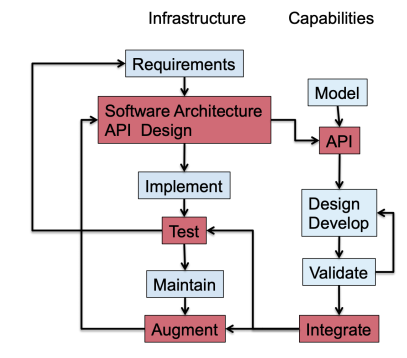
\includegraphics[width=281pt, height=253pt, keepaspectratio=true]{../png/wkflow.png}
%%\caption{This should be the caption for \texttt{M3.3.1-fig005.png}.}
%%\end{figure}

\label{HRef34587331}
\end{center}

\baselineskip=18pt
{ \textit{Figure 1: The design and development workflow between 
the Infrastructure and research model, taken from Ref~\cite{ref:8}.}}

On the left one can see that the infrastructure process model is structured and 
based upon requirements, while on right hand side, the model development can follow 
a more flexible, iterative process. As the model components mature, they are integrated 
into the infrastructure. It is good practice to use from the beginning improved 
design methods such as encapsulation, interfaces, separated units of computation, 
etc., to streamline development, avoid costly mistakes and to aid integration.

Because the models to be implemented are described by very complex sets of coupled 
equations, the design of the associate operators and data structures need careful 
attention. We have within our community a significant amount of experience around 
the BOUT++~\cite{ref:9} code, which implements various differential operators via C++ objects. 
BOUT++ is arguably the only state of the art tokamak turbulence code to have been 
developed from the ground up (primarily by the University of York). Most other turbulence 
codes developed in the UK have primary authors outside the UK in Europe or the 
US. Even more elaborate schemes that those exploited in BOUT++ are available in 
the literature, such as Arcos~\cite{ref:10}, which we plan to explore as the new edge models 
are significantly more complex than those that can currently be instantiated within 
the BOUT++ framework.

\section{Design for performance portability}

At the back end of the system, the separation of concerns methodology is also a 
useful approach for tackling hardware heterogeneity and rapid hardware evolution 
as vendors attempt to reduce the power overhead of exascale class archtectures. 
More often than not, in old software, numericaly intensive work is aggregated into 
a few large, monolithic tasks usually expressed as ``loop nests'' which can contain 
a large number of physical operators acting upon the whole discretised domain associated 
with a given MPI task. In order to ensure portability of numerical performance, 
without running into a combinatorial explosion of code versions, these large tasks 
should be partitioned using a new abstraction layer in which work is split into 
functional units and into chunks of the domain mapped to local memory. This layer 
must use the dependency inversion pattern~\cite{ref:11} to decouple its logic from the implementation 
logic which in turn can implemented with code generators and schedulers for a given 
hardware architecture, e.g. Kokkos,~\cite{ref:12} RAJA~\cite{ref:13} , SYCL~\cite{ref:14} etc.
The exploration 
of these technologies is a specific task of Activity~3. These methods are actively 
being explored by computational scientists and engineers across the UK HPC community. 
For \nep, we plan to have a dedicated collaboration in this field with one of 
the most qualified groups in UK.

\section{The Design pattern for the European Boundary Code}

As an example of the application of this methodology, we describe the top level 
design agreed for the first prototype of the European Boundary Code (EBC), being 
developed in parallel with \nep \   and in collaboration with UKAEA. 

The EBC will implement an ``extended fluid model'' which will couple multi-component 
plasma to neutrals and will be discretised over an unstructured grid using the 
discontinuous Galerkin method. As the model equations are not fully defined yet, 
and also the unstructured mesh and the discretisation for the tokamak geometry 
is not fully analysed, it was decided to explore the design space for a 2D reduced 
model using an infrastructure for the solvers and time evolution based upon exiting 
frameworks: PETSc~\cite{ref:15} for the solvers and the SUNDIALS~\cite{ref:16} suite for time integration. 
As these two frameworks have been used extensively by other plasma simulation codes, 
there is confidence from the accumulated expertise across Europe that they can 
be used for the new model/code without any forseable major problems. As these frameworks 
can be used at scale on modern HPC systems, they are also useful to establish a 
performance baseline for future optimisation and other more ambitious edge plasma 
codes. It is noteworthy to mention here that PETSc can exploit GPUs and so offers 
the possibility of a quick exploration of accelerator hardware for the candidate 
problems with a minimum of development time.

%\section{Bibliography}
\begin{thebibliography}{1}
\bibitem{ref:1}
O. O. Luk, O. Hoenen, A. Bottino, B. D. Scott and D. P. Coster
``ComPat framework for multiscale simulations applied to fusion plasmas, ''
\textit{Computer Physics Communications, }vol. 239, pp. 126-133, 2019. 

\bibitem{ref:2}
S. Longshaw, A. Skillen, C. Moulinec and D. R. Emerson,
``Code Coupling At Scale: Towards The Digital Product,''
in \textit{Advances in Parallel, Distributed, Grid and Cloud Computing for Engineering}, Saxe-Coburg Publications, Stirlingshire, UK, 2017. 

\bibitem{ref:3}
 J. Y. Choi, J. Logan, K. Mehta, E. Suchyta, W. Godoy, N. Thompson, L. Wan, 
J. Chen, N. Podhorszki, M. Wolf, S. Klasky, J. Dominski and C.-S. Chang,
``A Co-Design Study Of Fusion Whole Device Modeling Using Code Coupling,'' 2019. 
\newblock \url{: https://sc19.supercomputing.org/proceedings/workshops/workshop\_files/ws\_drbsd108s1-file1.pdf}

\bibitem{ref:4}
 S. D. Pinches,
``PROGRESS IN THE ITER INTEGRATED MODELLING PROGRAMME AND THE ITER SCENARIO DATABASE,'' 2018. 
\newblock \url{: https://nucleus.iaea.org/sites/fusionportal/Shared\%20Documents/FEC\%202018/fec2018-preprints/preprint0741.pdf}

\bibitem{ref:5}
``OMFIT,''
\newblock \url{: https://omfit.io/index.html}

\bibitem{ref:6}
R. Stevens, V. Taylor, J. Nichols, Maccabe, A. Barney, K. Yelick and D.  Brown, 
`AI for Science,''
Department of Energy, 2019.

\bibitem{ref:7}
 M. F. Kasim, D. Watson-Parris, L. Deaconu, S. Oliver, P. Hatfield, D. H. 
Froula, G. Gregori, M. Jarvis, S. Khatiwala, J. Korenaga, J. Topp-Mugglestone, 
E. Viezzer and S. M. Vinko,
``Up to two billion times acceleration of scientific simulations with deep neural architecture search,''
January 2020.
\newblock \url{: https://arxiv.org/abs/2001.08055}

\bibitem{ref:8}
A. Dubey,
``Software Design and Testing,'' 2019. 
\newblock \url{: https://extremecomputingtraining.anl.gov/files/2019/08/ATPESC\_2019\_Track-7\_3\_8-8\_1015am\_Dubey-Software\_Design\_and\_Testing.pdf}

\bibitem{ref:9}
``BOUT++,'' Available: https://boutproject.github.io/.

\bibitem{ref:10}
E. T. Coona, J. D. Moulton and S. L. Painter,
``Managing Complexity in Simulations of Land Surface and Near-surface Processes,''
\textit{Environmental Modelling and Software, }vol. 78, 2016. 

\bibitem{ref:11}
``Dependency inversion principle,'' 
\newblock \url{: https://en.wikipedia.org/wiki/Dependency\_inversion\_principle}

\bibitem{ref:12}
``Kokkos C++ Performance Portability Programming EcoSystem,'' 
\newblock \url{: https://github.com/kokkos/kokkos}

\bibitem{ref:13}
``RAJA,'' 
\newblock \url{: https://raja.readthedocs.io/en/master/}

\bibitem{ref:14}
``SYCL,'' 
\newblock \url{: https://www.khronos.org/sycl/}

\bibitem{ref:15}
``PETSc,'' 
\newblock \url{: https://www.mcs.anl.gov/petsc/}

\bibitem{ref:16}
``SUNDIALS: SUite of Nonlinear and DIfferential/ALgebraic Equation Solvers,''
\newblock \url{: https://computing.llnl.gov/projects/sundials}

\end{thebibliography}


\end{document}
